% -----------------------------------------------------------------
% Document class: Article
\documentclass[ a4paper, twoside, 11pt]{article}
\usepackage{../../../macros-general}
\usepackage{../../../macros-article}
% Number of the handout, quiz, exam, etc.
\newcommand{\numero}{01}
\setcounter{numero}{\numero}

% -----------------------------------------------------------------
\begin{document}
\allowdisplaybreaks

\begin{center}
\Large Mec\'anica Vectorial (MECG-1001): Lecci\'on \numero \\[2ex]
\small \textbf{Semestre:} 2017-2018 T\'ermino II \qquad
\textbf{Instructor:} Luis I. Reyes Castro \qquad
\textbf{Paralelo:} 08
\end{center}
\fullskip

% =============================================
\begin{problem}
Para la armadura mostrada en la siguiente figura (lado izquierdo):
\begin{enumerate}[label=\textbf{\alph*)}]
\item \textbf{3 Puntos:} Utilizando el m\'etodo de las secciones escriba tres ecuaciones de las cuales se puedan resolver para las fuerzas en los miembros $AB$, $AG$ y $FG$. \\[1ex] \emph{Soluci\'on:} Primero definimos: 
\[
\theta_{AB} \; = \; \arctan( 9 / 40 ) \; = \; 12.68\deg \qquad \qquad
\theta_{AG} \; = \; \arctan( 9 / 12 ) \; = \; 36.87\deg
\]
Luego, considerando la secci\'on $BCDGH$ tenemos: 
\begin{align*}
\sum F_x \; \colon \;
& +F_{AB} \, \cos(\theta_{AB}) + F_{AG} \, \cos(\theta_{AG}) + F_{FG} \; = \; 0 \\[1ex]
\sum F_y \; \colon \;
& -F_{AB} \, \sin(\theta_{AB}) - F_{AG} \, \sin(\theta_{AG}) - 4.5 \; = \; 0 \\[1ex]
\sum M_G \; \colon \;
& - (9) \, ( 1 - 12/40 ) \, F_{AB} \, \cos(\theta_{AB}) - (14)(1.8) - (28)(0.9) \; = \; 0
\end{align*}

\item \textbf{1.5 Puntos:} Calcule las fuerzas en los miembros $AB$, $AG$ y $FG$. Por favor denote fuerzas de compresi\'on con signo positivo y de tensi\'on con signo negativo. \\[1ex] \emph{Soluci\'on:} De la sumatoria de momentos en $G$ obtenemos:
\[
F_{AB} = -8.2 \text{ kips}
\]
Luego, de la sumatoria de fuerzas en $y$ obtenemos: 
\[
F_{AG} = -4.5 \text{ kips}
\]
Finalmente, de la sumatoria de fuerzas en $x$ obtenemos: 
\[
F_{FG} = +11.6 \text{ kips}
\]

\item \textbf{3 Puntos:} Utilizando el m\'etodo de las secciones escriba tres ecuaciones de las cuales se puedan resolver para las fuerzas en los miembros $AE$, $EF$ y $FJ$. \\[1ex] \emph{Soluci\'on:} Primero definimos: 
\[
\theta_{AE} \; = \; \arctan( 9 / 8 ) \; = \; 48.37\deg
\]
Luego, considerando la secci\'on $ABCDFGH$ tenemos: 
\begin{align*}
\sum F_x \; \colon \;
& +F_{AE} \, \cos(\theta_{AE}) + F_{EF} \; = \; 0 \\[1ex]
\sum F_y \; \colon \;
& +F_{AE} \, \sin(\theta_{AE}) + F_{FJ} - 5.4 \; = \; 0 \\[1ex]
\sum M_A \; \colon \;
& +9 \, F_{EF} - (12)(1.8) - (26)(1.8) - (40)(0.9) \; = \; 0
\end{align*}

\item \textbf{1.5 Puntos:} Calcule las fuerzas en los miembros $AE$, $EF$ y $FJ$. \\[1ex] \emph{Soluci\'on:} De la sumatoria de momentos en $A$ obtenemos:
\[
F_{EF} = +11.6 \text{ kips}
\]
Luego, de la sumatoria de fuerzas en $x$ obtenemos: 
\[
F_{AE} = -17.46 \text{ kips}
\]
Finalmente, de la sumatoria de fuerzas en $y$ obtenemos: 
\[
F_{FJ} = +18.45 \text{ kips}
\]

\end{enumerate}

\end{problem}
\fullskip

% =============================================
\begin{problem}
Para el armaz\'on mostrado en la siguiente figura (lado derecho):
\begin{enumerate}[label=\textbf{\alph*)}]
\item \textbf{2 Puntos:} Bosqueje los diagramas de cuerpo libre de las barras $ABC$ y $DEF$. \\[1ex] \emph{Soluci\'on:} Definiendo $\theta = \arctan( 15 / 20 ) = 36.87\deg$, tenemos: 
\begin{itemize}
\item Cuerpo $ABC$: 
\begin{align*}
\sum F_x \; \colon \;
& -F_{AD} \, \cos(\theta) - F_{BE} \, \cos(\theta) + C_x + 100 \; = \; 0 \\[1ex]
\sum F_y \; \colon \;
& +F_{AD} \, \sin(\theta) + F_{BE} \, \sin(\theta) + C_y \; = \; 0 \\[1ex]
\sum M_C \; \colon \;
& +45 \, ( \, F_{AD} \, \cos(\theta) - 100 \, ) + 30 \, F_{BE} \, \cos(\theta) \; = 0
\end{align*}
\item Cuerpo $DEF$: 
\begin{align*}
\sum F_x \; \colon \;
& +F_{AD} \, \cos(\theta) + F_{BE} \, \cos(\theta) + F_x \; = \; 0 \\[1ex]
\sum F_y \; \colon \;
& -F_{AD} \, \sin(\theta) - F_{BE} \, \sin(\theta) + F_y \; = \; 0 \\[1ex]
\sum M_F \; \colon \;
& -30 \, F_{AD} \, \cos(\theta) - 15 \, F_{BE} \, \cos(\theta) \; = 0
\end{align*}
\end{itemize}

\item \textbf{2 Puntos:} Calcule las fuerzas en los eslabones $AD$ y $BE$. Por favor denote fuerzas de compresi\'on con signo positivo y de tensi\'on con signo negativo. \\[1ex] \emph{Soluci\'on:} Considerando el cuerpo $DEF$ y sumando de momentos en $F$ tenemos: 
\[
F_{BE} = -2 \, F_{AD}
\]
Luego, considerando el cuerpo $ABC$ y sumando momentos en $C$ tenemos: 
\begin{align*}
& +45 \, ( \, F_{AD} \, \cos(\theta) - 100 \, ) - 60 \, F_{AD} \, \cos(\theta) \; = 0 \\
& \Longrightarrow \;
F_{AD} \; = \; -375 \text{ lb}, \;
F_{BE} \; = \; +750 \text{ lb}
\end{align*}

\item \textbf{2 Puntos:} Calcule las reacciones en $C$ y $F$. \\[1ex] \emph{Soluci\'on:} Considerando el cuerpo $ABC$ y sumando fuerzas tenemos: 
\[
C_x \; = \; +200 \text{ lb}, \quad
C_y \; = \; -225 \text{ lb}
\]
Luego, Considerando el cuerpo $DEF$ y sumando fuerzas tenemos: 
\[
F_x \; = \; -300 \text{ lb}, \quad
F_y \; = \; +300 \text{ lb}
\]

\end{enumerate}

\begin{figure}[htb]
\centering
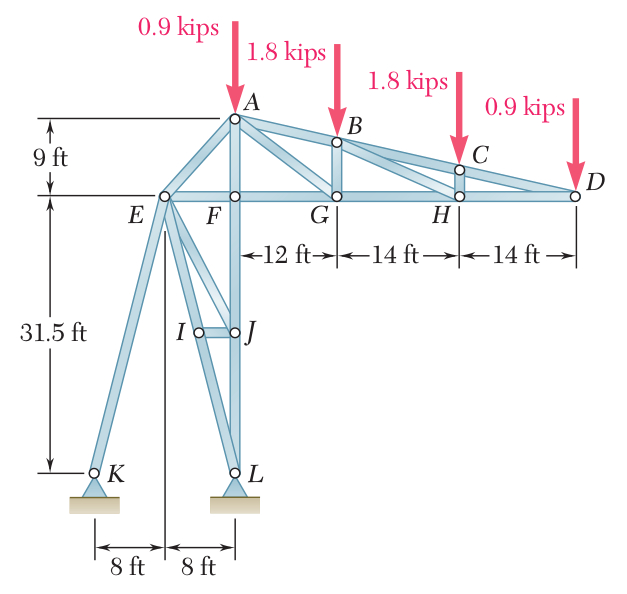
\includegraphics[width=0.56\textwidth]{prob-armadura.jpg} \qquad
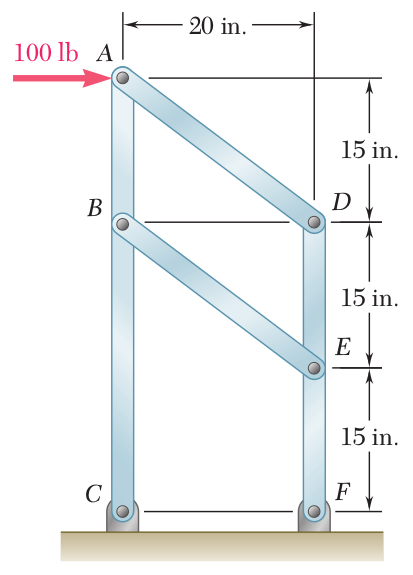
\includegraphics[width=0.32\textwidth]{prob-armazon.jpg}
\end{figure}

\end{problem}
\fullskip

% =============================================
\begin{problem}
Una barra delgada $AB$ de peso $W$ se une a los bloques $A$ y $B$ que se mueven libremente sobre las gu\'ias como se muestra en la siguiente figura. El resorte, que tiene una constante $k$, se encuentra sin deformar cuando $\theta = 0\deg$. 
\begin{enumerate}[label=\textbf{\alph*)}]
\item \textbf{3 Puntos:} Sin tomar en cuenta el peso de los bloques, encuentre una ecuaci\'on en t\'erminos de $W$, $k$, $l$ y $\theta$ que se cumpla cuando la barra est\'a en equilibrio. 
\item \textbf{3 Puntos:} Determine el valor de $\theta$ cuando $W = 75$ lb, $l = 30$ in y $k = 3$ lb/in. 
\end{enumerate}

\begin{figure}[htb]
\centering
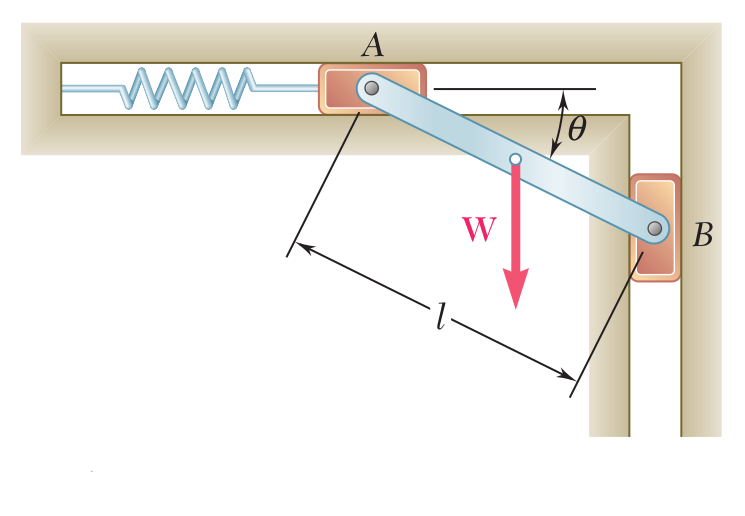
\includegraphics[width=0.42\textwidth]{prob-equilibrio.jpg}
\end{figure}

\end{problem}
\fullskip

% =============================================
\begin{problem}
\textbf{4 Puntos:} Para la viga mostrada en la siguiente figura encuentre la fuerza cortante $V(x)$ y el momento flector $M(x)$ como funci\'on de la posici\'on $x \in [0,4]$. 

\begin{figure}[htb]
\centering
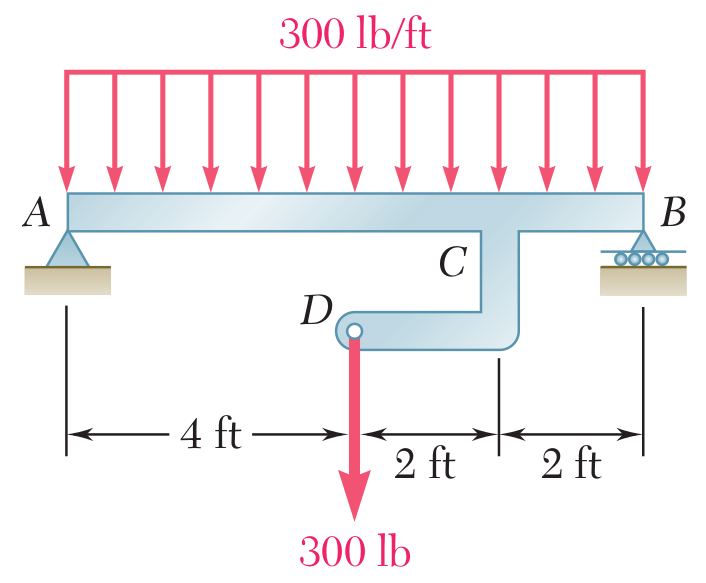
\includegraphics[width=0.36\textwidth]{prob-vigas.jpg}
\end{figure}

\end{problem}
\fullskip

\end{document}